\documentclass{entry}

\title{卒業研究審査登録書の書式}
\author{G984822019}{吉村 直将}
\supervised{
	\supervisor{教授}{蓑原 隆}
	\supervisor{助手}{田島 信行}
}
\begin{document}
\maketitle

\section{はじめに}
\subsection{研究背景}
近年,サイバー攻撃の発生件数が年々増加してきており,その攻撃手法も多様化している.
対策として,攻撃者を誘き寄せ,
不正アクセスを受けるハニーポットを運用し,
攻撃者の情報を収集してきた.過去の研究では,
ハニーポットを利用して,
ログイン試行時に使われるIDやパスワード,
ログイン後に攻撃者から送られるシェルコマンド等の情報を収集し,研究を行ってきた.
得られる情報の中でログイン後に送られるコマンドを解析することは、
攻撃者がログイン成功後にどうゆう意図で,何を目的をとして攻撃を行なってくるかの予測が立てらる.
又,コマンドから攻撃者がダウンロードさせようとしてくる不正なソフトウェアの情報を知り、調査できる為,
より最新の攻撃に対して具体的なセキュリティ対策につながると思われる.

\subsection{攻撃ホストからハニーポットへの攻撃の流れ}
攻撃者ホストからハニーポットへの攻撃の流れとして図1に示してある.
攻撃ホストはハニーポットにログイン試行としてID/パスワードを送信してくる.
ハニーポットはそれに対して,ログイン許可をしている風に見せる,
攻撃者はログイン後操作する為に,コマンドを送信する.
この攻撃の中でハニーポットはログイン試行時に使われるIDやパスワード,
ログイン後に攻撃者から送られるシェルコマンド等の情報を収集し,
収集した情報から攻撃手法の研究してきた. 
\begin{figure}[htbp]
	\centering
	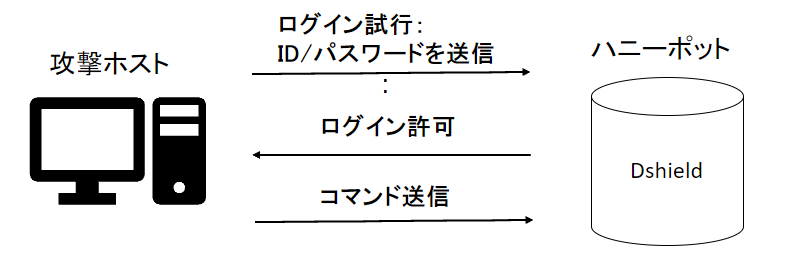
\includegraphics[width=\hsize]{honeypot1.png}
	\caption{攻撃の流れ}
\end{figure}
\subsection{目的}
本研究では,より具体的な攻撃者の攻撃手法の情報を得る為、攻撃者がログイン成功後に行う攻撃に着目し,
ハニーポットを用いることで,攻撃者から送信されるコマンドやそのコマンドから入手できるファイルの情報を収集し,
解析するシステムを構築する.そして,攻撃の分析を行い,最新の攻撃内容について警告を発することを目的とする。


\section{研究方法}
本研究では,ハニーポットDshieldを用いる.DShield(Distributed Intrusion Detection System)は,
グローバルなセキュリティコミュニティによって構築された分散型侵入検知システムである.
世界中のネットワーク上で発生するセキュリティイベントのデータを収集し,
分析することでセキュリティの脅威情報を提供する.Dshieldは研究室で以前から運用していたが,
ログイン試行時のIdやパスワードを収集することを目的としたハニーポットであった.
本研究では,ログイン後のコマンドを収集することが目的としている為,
新しくハニーポットを構築することとする.                 
本研究の目的である攻撃者がダウンロードさせようとしてくる
不正なソフトウェアの解析を実現する為のシステムを図2に示す.                   
ハニーポットはインターネットから攻撃受け,攻撃者からのコマンドを収集する.
コマンドから,不正なサイトで攻撃者がダウンロードさせてくるソフトウェアのデータを集めるプログラムを構築し,
不正なソフトウェアを解析するものを作る.     

研究計画として,
\begin{enumerate}
    \item Dshieldを運用できる環境を構築をする.
    \item コマンドを収集するために、Dshieldのプログラム内で、
	攻撃者からのコマンドに対してどのような動作をしているかを確認する.
    \item 実際にDshieldを運用してみる.
    \item 取集したコマンドの内容について調べる.
    \item コマンドからファイル又は,URLなどを取集するプログラムを作成する.
    \item ファイルがどのようなものなのか調べる.
\end{enumerate}
     という手順で進めていき,攻撃ファイルがどの様なものなのか把握し,
どのような対策が有効的なのか等の警告を発することで,セキュリティの向上に貢献していきたい.


\section{今まで行ってきたこと}
\subsection{Dhieldの運用できる環境の構築}
Raspberry PiにDshieldをインストールし,パスワードや接続する無線LANの設定を行なった.
設定の更新には,少しの時間が掛かっった.又,RassberryPiの設定からインターフェースのSSHを有効にする事で,
SSHを通って外部PCから接続を可能にした.研究室内のネットワークからの接続は攻撃と見さないように設定した.
\subsection{Dshieldが行う攻撃者のログイン試行への対処方法}
Dshieldは研究室で以前から運用されていたがidやパスワードの収集を目的として使われていた.本研究では、コマンドを収集したいので,
Dshieldのプログラム内容からコマンドを収集できているのか,又出来る様に設定していきたい.調査の結果,
Dshieldはコマンドを取集していることが分かった.収集したコマンドは,/srv/cowrie/var/log/cowrieの場所に保存されていることが分かった.
又,

\subsection{収集したコマンド内容と攻撃者の意図}


\section{今後やる事}



\bibliographystyle{entry}
%\bibliographystyle{junsrt}
\bibliography{sample}

\end{document}
